\documentclass{report}
\usepackage{imakeidx}
\usepackage[utf8]{inputenc}
\usepackage[english]{babel}
\usepackage[T1]{fontenc}
\usepackage{graphicx}
\graphicspath{{./}}
\usepackage{geometry}
\geometry{
a4paper,
margin=1in,left=1.25in,
}
\usepackage{tikz}
\usetikzlibrary{calc}
\usetikzlibrary{decorations.pathmorphing}
\usepackage{tikzpagenodes}
\usepackage{fancyhdr}
\pagestyle{fancy}
\fancyhead{}
\renewcommand{\headrulewidth}{1pt}
\renewcommand{\footrulewidth}{1pt}
\renewcommand{\baselinestretch}{1.5}

\begin{document}

\begin{titlepage}
\begin{center}
\centerline{
\includegraphics[width=2.5in,height=2in,keepaspectratio]{jssstu}}
\Large{\bfseries JSS Science And Technology University}\\
\Large{\bfseries Mysuru}\\
\Large{\bfseries 570 006}\\
[1cm]
\Large{\bfseries Department of Computer Science and Engineering}\\
[1cm]
\textsc{\LARGE The Report}\\
[1cm]	
\huge {\bfseries Drug Database and Rehabilitation Booking System}\\
[1cm]
\textsc{\LARGE Submitted By}\\
\large{\bfseries Nivedita M Hanamasagar}\\
\large{\bfseries Vaishnavi Srinath}\\
\large{\bfseries Chinmayi P}\\
\large{\bfseries Suma Y Gouda}\\
\large{\bfseries Sneha H}\\
\end{center}
\end{titlepage}

\renewcommand{\abstractname}
{\Large DECLARATION}
\title{DECLARATION}
\begin{abstract}
\vspace{1cm}

We, Nivedita Hanamasagar, Vaishnavi Srinath, Chinmayi P, Suma Y Gouda, Sneha H, declare that this dissertation is entirely our own original work and that, to the best of our knowledge, it has not been presented or submitted for any degree or examination in any other university, and that all the sources we have used or quoted have been indicated and acknowledged by complete references.\\
\textsc{\large PROJECT SUPERVISOR}\\
\large{\bfseries Name: Dr. Trisiladevi Nagavi}\\
\large{\bfseries Signature: ................}\\
\large{\bfseries Date: ..................}\\
\end{abstract}
\pagebreak

\tableofcontents
\chapter{Introduction}
\section{Objective of the project}
To create awareness among the common people about the use of illegal drugs and making it easy for them reach the de-addiction centers.
\section{Features of the project}  
The database:\\
Provides information about the following aspects related to drugs:
\begin{itemize}
\item Varieties of drugs.
\item Laws and policies against the use of banned drugs.
\item Availability of doping agencies around the world.
\item Disorders caused by the consumption of banned drugs.
\item Treatment for the disorders.
\item Availability of the rehabilitation homes for drug addicts. 
\item Role of drugs for treating covid-19.\\
\\
The website:
\item Provides access to the information about all the above aspects. 
\item Provides the service of booking of rehabilitation homes.
\\
Requirements:
\item Back end: MySql, PHP
\item Front end: HTML, CSS, Java Script 
\end{itemize}
\chapter{System Design}
\section{ER Diagram-high level data modeling}
\centerline{\includegraphics[width=7in,height=5in,keepaspectratio]{ER_Diagram}}
\section{Schema Diagram-conceptual data modeling}
\centerline{\includegraphics[width=7in,height=5in,keepaspectratio]{Relational_Schema}}
\section{State Diagram}
\centerline{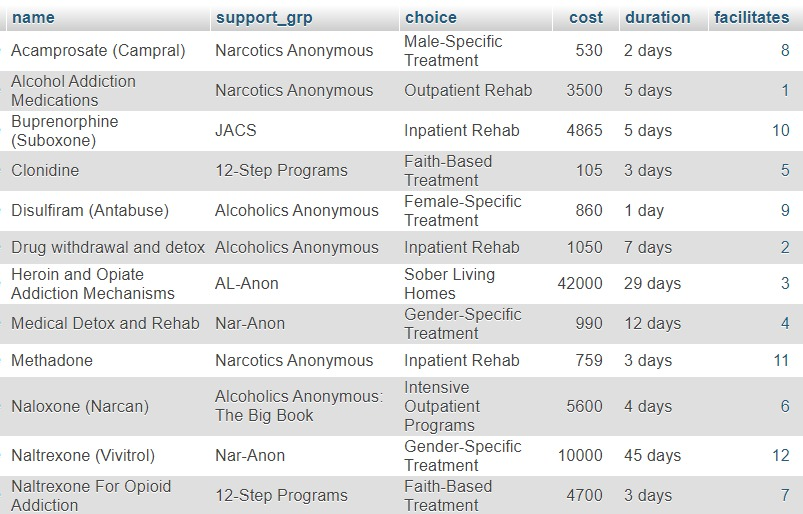
\includegraphics[width=7in,height=5in,keepaspectratio]{sd1}}\\
\centerline{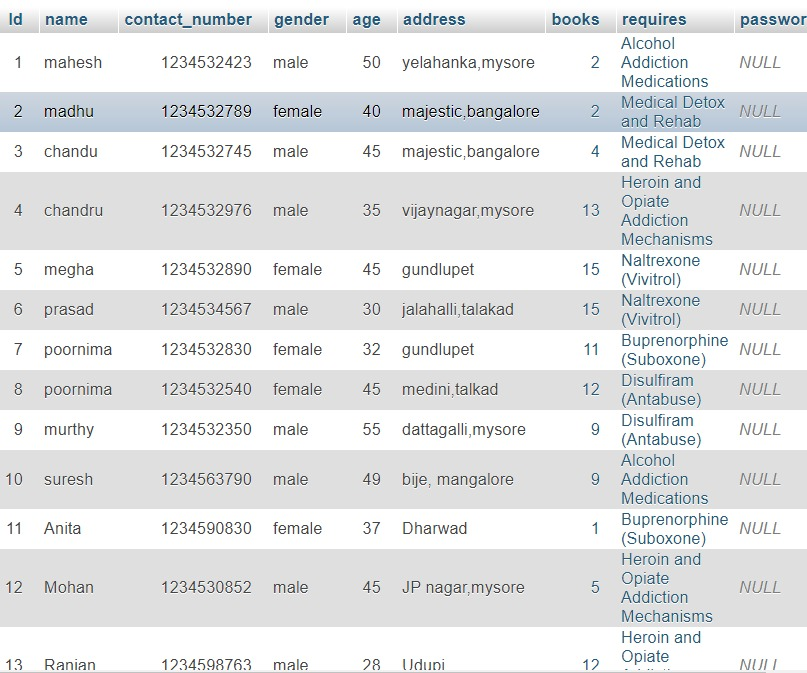
\includegraphics[width=7in,height=5in,keepaspectratio]{sd2}}\\
\centerline{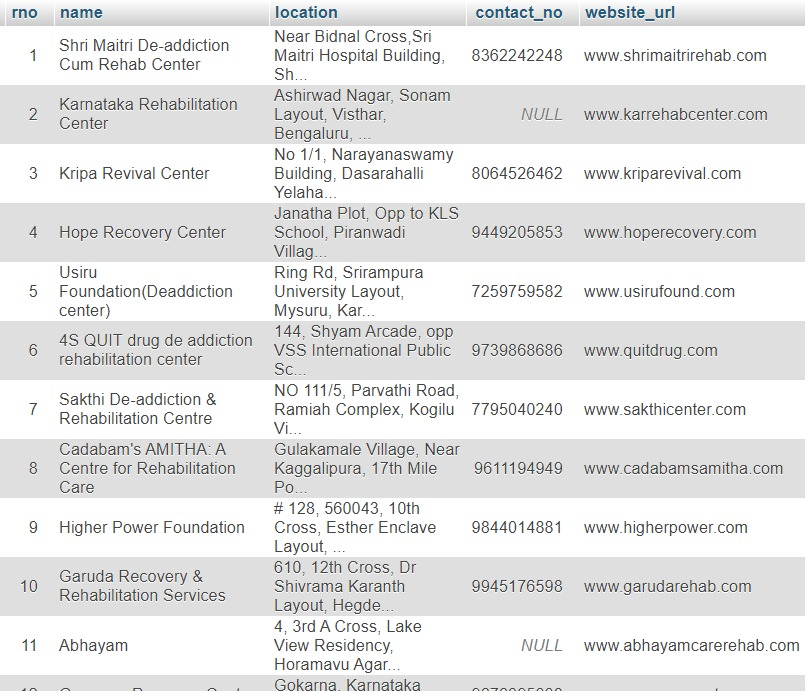
\includegraphics[width=7in,height=5in,keepaspectratio]{sd3}}\\
\centerline{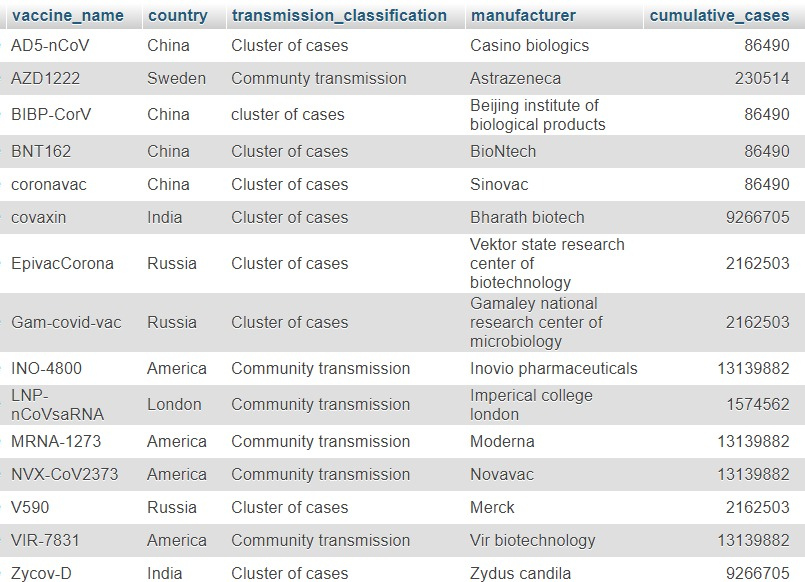
\includegraphics[width=7in,height=5in,keepaspectratio]{sd4}}\\
\centerline{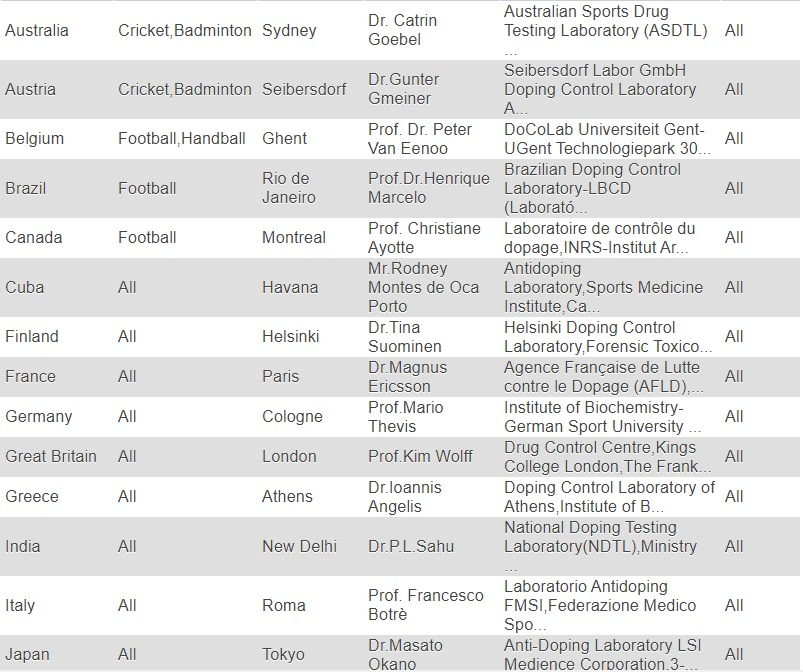
\includegraphics[width=7in,height=5in,keepaspectratio]{sd5}}\\
\chapter{Normalization upto 3 NF}
\hspace{0.5cm} \textbf{1NF:}
Each column should contain atomic values
     Entries like x,y, and w,x violate this rule.
The column should contain values that are of the same type.
     Do not intermix different types of values in any column.
Each column should have a unique name 
      Same names lead to confusion at the time of data retrieval.
The order in which data is saved doesn’t matter
                 Using SQL query you can easily fetch data in any order from a table.

\textbf{2NF:}
Second Normal Form (2NF) is based on the concept of fully functional dependency. Second Normal Form applies to relations with composite keys, that is, relations with a primary key composed of two or more attributes. A relation with a single-attribute primary key is automatically in at least 2NF. A relation that is not in 2NF may suffer from the update anomalies.
To be in second normal form, a relation must be in first normal form and the relation must not contain any partial dependency. A relation is in 2NF if it has No Partial Dependency, i.e., no non-prime attribute (attributes which are not part of any candidate key) is dependent on any proper subset of any candidate key of the table.

\textbf{3NF:}
A relation will be in 3NF if it is in 2NF and no transition dependency exists.
    A relation is in third normal form if there is no transitive dependency for non-prime attributes as well as it is in second normal form.
A relation is in 3NF if at least one of the following condition holds in every non-trivial function dependency X –> Y:
X is a super key.
Y is a prime attribute (each element of Y is part of some candidate key).

As there are 3 techniques to achieve First Normal Form, we opted for technique in which a multivalued or a composite attribute is divided into atomic attributes.
As there was no functional dependency and transitive dependency, it was already in Second and Third Normal Form.
\chapter{System Implementation}
\section{Introduction to MySQL and DBMS}
\hspace{0.5cm} \textbf{MySQL} is a popular open-source relational database management system (RDBMS) that is developed,
distributed and supported by Oracle Corporation.
In MySQL, each individual records are stored as ‘rows’ in a table.
A ‘table’ is used to store rows (records) of similar type.
MySQL as the name suggests uses Structured Query Language (SQL) for database access. 
The schema can not be changed. The inputs following the given schema are only entered.

A \textbf{Database management system (DBMS)} refers to the technology for creating and managing databases. 
DBMS is a software tool to organize (create, retrieve, update, and manage) data in a database.
The main aim of a DBMS is to supply a way to store up and retrieve database information that is both 
convenient and efficient. By data, we mean known facts that can be recorded and that have embedded meaning. Usually, people use software such as DBASE IV or V, Microsoft ACCESS, or EXCEL to store data in the form of a database. A datum is a unit of data. Meaningful data combined to form information.

\textbf{Why we used MySQL is because} MySQL is well-organized for its high performance,flexibility,reliable data protection,high availability and management ease. Proper data indexing can solve the issue with performance, facilitates interaction and ensure robustness. MySQL features a distinct storage-engine framework that facilitates system administrators to configure the MySQL database server for a flawless performance. It comes with the assurance of 24*7 uptime and offers a wide range of high availability solutions. With the average download and installation time being less than 30 minutes, MySQL means usability from day one. All the fears and worries that arise in an open source solution can be brought to an end with MYSQL’s round-the-clock support. By considering all the above mentioned features we decided to use MySQL.
\section{Relational Algebraic Queries}
\begin{itemize}
\item Select\\
select * from covid\_19 where country="india";\\
\item Project\\
select distinct Country,Name from laws;\\
\item Set Union\\ 
select Country from agency where Games='Football' union select Country from laws\\
        where Year\_of\_enforcement>2000;\\
\item Set Intersection\\
select id,patient,name,gender,age,requires from patient left join treatment on\\ 
    patient.requires=treatment.name;\\
\item Set Difference\\
select adress from patient where not exists(select location from rehabs where \\
        patient.adress=rehabs.location);\\
\item Cross Product\\
select rehabs.rno,rehabs.name, cured\_by.disorder\_number,cured\_by.rno from rehabs\\ 
        cross join cured\_by;\\
\item Rename\\
select A.Games as Sports, A.Lab\_Head as Laboratory\_Incharge, A.Address as Location,\\ 
        A.doping as Tests from agency as A where A.Games="Football";\\
\end{itemize}
\section{Queries designed using SQL commands}
\renewcommand{\labelenumii}{\Roman{enumii}}
\begin{enumerate}
\item SIMPLE:
    \begin{itemize}
        \item desc laws;
        \item select * from drug\_varieties;
        \item update treatment set cost=10000 where duration='45 days';
        \item alter table unwanted add useless int;
        \item alter table unwanted drop column useless;
        \item create table covid\_19(vaccine\_name varchar(20), country char(20), transmission\_classification char(25), manufacturer char(25), cumulative\_cases bigint, primary key(vaccine\_name));
        \item delete from disorders where disorder\_name='Ataxia';
        \item create table var\_category(Variety\_number int, category varchar(20), primary key(Variety\_number),\\
                foreign key(Variety\_number) references drug\_varieties(Variety\_number) on delete cascade);
    \end{itemize}
\item NESTED:
    \begin{itemize}
        \item select Disorder\_number from disorders where Disorder\_number in (select rno from cured\_by where cured\_by.rno=5);
        \item select name from rehabs where rno in (select Disorder\_number from cured\_by where cured\_by.Disorder\_number>2);
        \item select * from treatment where facilitates in (select rno from rehabs where name='Kripa Revival Center');
        \item select Country from laws where Name in (select Name from restricts\_to);
        \item select Country from laws where Name in (select Name from restricts\_to where Variety\_number<5);
    \end{itemize}
\item SET operations:
    \begin{itemize}
        \item select Country from agency where Games='Football' union select Country from laws where Year\_of\_enforcement>2000;
        \item select distinct Caused\_by from disorders where Caused\_by in (select Category from drug\_varieties);
    \end{itemize}
\item GROUP BY:
    \begin{itemize}
        \item select count(cumulative\_cases),transmission\_classification from covid\_19 group by transmission\_classification;
        \item select country,count(*) from covid\_19 group by country;
    \end{itemize}
\item ORDER BY:
    \begin{itemize}
        \item select variety\_number,example\_1 from drug\_varieties order by variety\_number;
    \end{itemize}
\item CHECK:
    \begin{itemize} 
        \item alter table covid\_19 add check(cumulative\_cases>=20000);
    \end{itemize}
\item HAVING:
    \begin{itemize}
        \item select * from treatment having cost>1000;
    \end{itemize}
\item EXISTS and NOT EXISTS:
    \begin{itemize}
        \item select adress from patient where not exists(select location from rehabs where\\
                patient.adress=rehabs.location);
        \item select vaccine\_name from covid\_19 where exists(select vaccine\_name from updates\_on);
    \end{itemize}
\item Aggregate functions:
    \begin{itemize}
        \item select count(distinct City) from agency where Games='All';
        \item select sum(cost) from treatment;
        \item select max(cumulative\_cases) as MAX\_CASES from covid\_19;
        \item select min(cumulative\_cases) as MIN\_CASES from covid\_19;
        \item select avg(cumulative\_cases) as AVG\_CASES from covid\_19;
    \end{itemize}
\item Like, Between:
    \begin{itemize}
        \item select Substance,Sweat from detected where Sweat like '\%days';
        \item select name,contact\_no from rehabs where contact\_no like '9\_\_\_\_\_\_\_\_\_';
        \item select name,age from patient where age between 18 and 50;
    \end{itemize}
\item Correlated queries:
    \begin{itemize}
        \item select name from patient where age>30 and exists (select * from patient);
        \item select country from covid\_19 where cumulative\_cases > (select avg(cumulative\_cases) from covid\_19 where vaccine\_name=vaccine\_name);  
    \end{itemize}
\item Views:
    \begin{itemize}
        \item create view patient\_rehab\_treatment(Patient\_Name, Rehab\_Name, Treatment\_Name,
                Treatment\_Choice) as select p.name, r.name, t.name, t.choice from patient as p, 
                rehabs as r, treatment as t where p.books=r.rno and p.requires=t.name;
    \end{itemize}
\item Triggers:
    \begin{itemize}
        \item create trigger upcase before insert on patient for each row set new.Name=upper(new.Name);
    \end{itemize}
\item Stored Procedures:
    \begin{itemize}
        \item create procedure SelectAllRehabs() select * from rehabs go;
        \item call SelectAllRehabs;
    \end{itemize}
\end{enumerate}
\chapter{System Testing and Results}
\section{Architectural Design}
The design of DBMS depends on its architecture. DBMS architecture helps in design, development, implementation, and maintenance of a database. A database stores critical information for a business. Selecting the correct Database Architecture helps in quick and secure access to this data.
Architectural design elements give us an overall view of the software.It involves identifying
the major components of the system and the communication between these components.The architectural design element is usually depicted as a set of interconnected subsystems, often derived from analysis packages within the requirements model. ArchitecturalStyle: Our software is based on data centered architecture.

 All the modules or components access this repository to store,retrieve or manipulate data as a result of which any changes made to the database will be updated and this updated version is available to all modules. Main purpose of data centered architecture is to achieve integrality of data. Data-centered architecture consists of different components that communicate through shared data repositories. The components access a shared data structure and are relatively independent, in that, they interact only through the data store.
We are using mysql in the backend which acts as the data repository for our drug database. we can interact with this database to insert , update and delete data in the database. The data is consistent and integrality of data is also maintained. We are making use of mysql,phpmyadmin for backend and html,css with bootstrap framework for frontend design.
\centerline{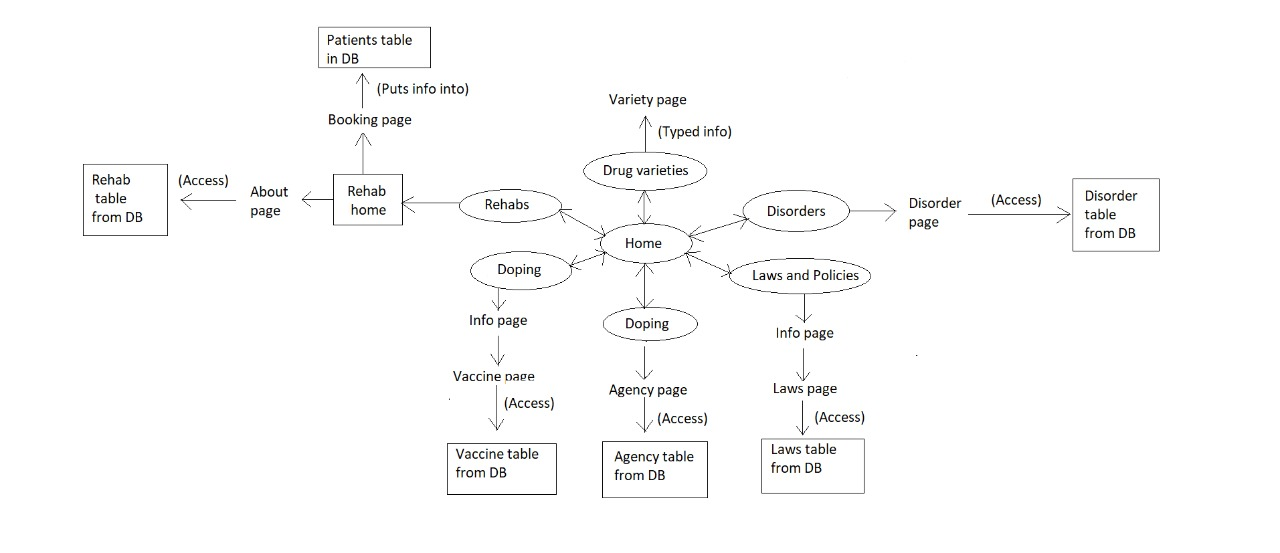
\includegraphics[width=7in,height=5in,keepaspectratio]{design1}}\\
\section{Graphical Description of Web Pages}
[1cm]
\centerline{\includegraphics[width=7in,height=5in,keepaspectratio]{w1}}\\
[1cm]
\centerline{\includegraphics[width=7in,height=5in,keepaspectratio]{w2}}\\
[1cm]
\centerline{\includegraphics[width=7in,height=5in,keepaspectratio]{w3}}\\
\section{Unit Testing and Results}
Unit testing is a testing method which allows us to test the smallest,atomic programmable part of a
database object. Using the component-level design description as a guide, important control paths are
tested to uncover errors within the boundary of the module. This testing plays a key role in the modern
database development. Unit testing adds a great worth to database project because unit tests are more
reliable than manual test methods. It focuses on the internal processing logic and data structures within
the boundaries of a component. In this portion of the report, we unveil various tests on the module and the
features  in response.\\
\begin{center}
\centerline{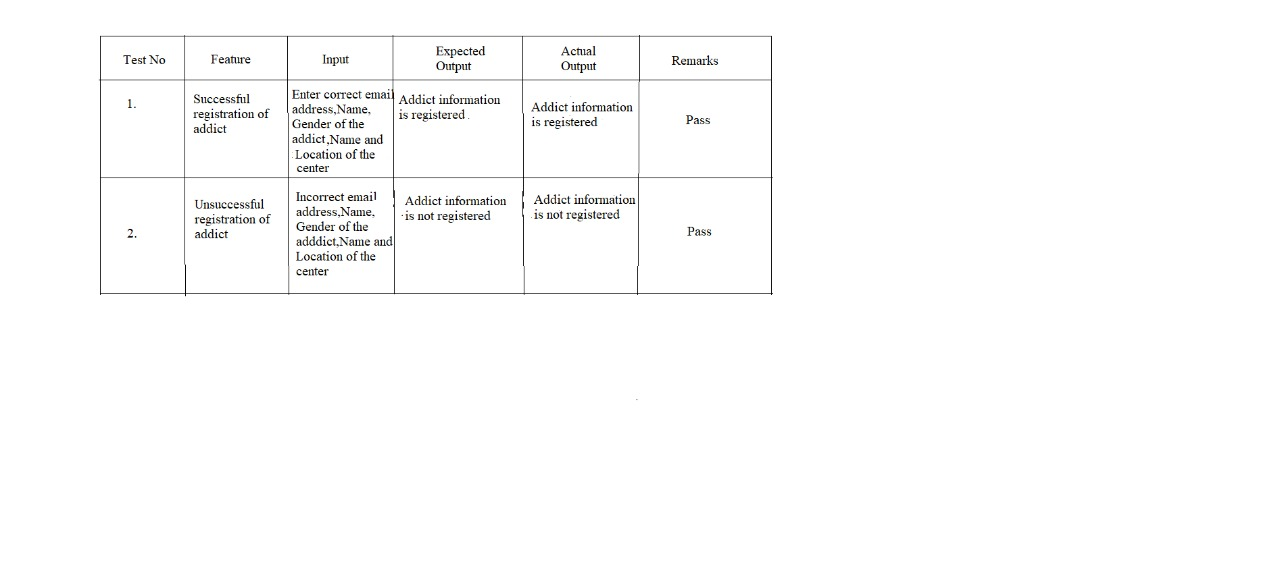
\includegraphics[width=7in,height=5in,keepaspectratio]{test_results}}\\
\end{center}
\chapter{Conclusion}
This report attempted to provide a brief visualisation of the project \textbf{Drug Database}. Addiction doesn’t discriminate, and it affects all types of people from different backgrounds. Being aware of the issue allows 
people from all walks of life to open up.  Many people fall into the delusion that addiction only happens to people who live in certain parts of the country or have specific backgrounds. However, the truth of the matter is that addiction is a disease. 
This disease hurts people from all walks of life, some are just better at hiding it. We want anyone struggling with addiction to feel comfortable opening up. Opening up about the issue is the first step in choosing to live a better, sober life. In order to maintain a healthy society, this step of making a website that helps people become aware of drugs and also allowing them to book a rehabilitation center for their loved ones is taken.

ER Diagram and Relational Schema(as shown in section 2.1 and 2.2) were first developed in order to have clear idea of the project. Then we achieved Normalisation upto 3NF. Later we executed SQL queries(mentioned in section 4.2 and 4.3)
in phpmyadmin and MySQL command line interface. For backend we used PHP, MySQL, MAMP server whereas for forntend we used HTML, CSS, Bootstrap and Javascript.
\chapter{References}
\begin{itemize} 
\item Fundamentals of Database Systems
    \begin{itemize}
        \item Ramez Elmasri and Shamkant B. Navathe
    \end{itemize}
\item www.w3schools.com
    \begin{itemize}
        \item For learning HTML and Bootstrap
    \end{itemize}
\item www.stackoverflow.com
    \begin{itemize}
        \item For doubts clarification
    \end{itemize}
\item https://youtu.be/4q0gYjAVonI
    \begin{itemize}
        \item For PHP
    \end{itemize}
\item https://youtu.be/4q0gYjAVonI
    \begin{itemize}
        \item For Backend
    \end{itemize}
\item https://www.youtube.com/watch?v=OOy764mDtiA&ab_channel=DaniKrossing
    \begin{itemize}
        \item For Frontend
    \end{itemize}
\end{itemize}
\printindex
\end{document}